%!TEX TS-program = xelatex
\documentclass[12pt, a4paper, oneside]{article}

\usepackage{amsmath,amsfonts,amssymb,amsthm,mathtools}  % пакеты для математики

\usepackage[english, russian]{babel} % выбор языка для документа
\usepackage[utf8]{inputenc} % задание utf8 кодировки исходного tex файла
\usepackage[X2,T2A]{fontenc}        % кодировка

\usepackage{fontspec}         % пакет для подгрузки шрифтов
\setmainfont{Linux Libertine O}   % задаёт основной шрифт документа

\usepackage{unicode-math}     % пакет для установки математического шрифта
%\setmathfont[math-style=upright]{Neo Euler} % шрифт для математики

% Размер страницы 
\usepackage[paper=a4paper, top=20mm, bottom=15mm,left=20mm,right=15mm]{geometry}
\usepackage{indentfirst}       % установка отступа в первом абзаце главы

\usepackage{setspace}
\setstretch{1.1}  % Межстрочный интервал
\setlength{\parskip}{4mm}   % Расстояние между абзацами
% Разные длины в латехе https://en.wikibooks.org/wiki/LaTeX/Lengths

\pagestyle{empty}

% Работа с картинками
\usepackage{graphicx}                  % Для вставки рисунков
\usepackage{graphics}
\graphicspath{{images/}}    % можно указать папки с картинками
\usepackage{wrapfig}                   % Обтекание рисунков и таблиц текстом
\usepackage{float}    

% Более-менее приятный синий, который не режет глаза
\usepackage{xcolor}
\definecolor{myblue}{rgb}{0.1, 0.45, 0.70}

% Немного подрифтуем списки и расстояния в них 
\usepackage{enumitem}
\newcommand*{\MyPoint}{\tikz \draw [baseline, fill=myblue,draw=blue] circle (2.5pt);}
\renewcommand{\labelitemi}{\MyPoint}

\setlist[itemize]{parsep=0.4em,itemsep=0em,topsep=0ex}
\setlist[enumerate]{parsep=0.4em,itemsep=0em,topsep=0ex}


% Работа с гиперссылками 
\usepackage{hyperref}
\hypersetup{
	unicode=true,           % позволяет использовать юникодные символы
	colorlinks=true,       	% true - цветные ссылки, false - ссылки в рамках
	urlcolor=blue,          % цвет ссылки на url
	linkcolor=red,          % внутренние ссылки
	citecolor=green,        % на библиографию
	pdfnewwindow=true,      % при щелчке в pdf на ссылку откроется новый pdf
	breaklinks              % если ссылка не умещается в одну строку, разбивать ли ее на две части?
}



% Счётчик для задачек 
\newcounter{problem}
\renewcommand{\theproblem}{\arabic{problem}}
\newcommand{\problemname}{Задача}

\newenvironment{problem}{
	\addtocounter{problem}{1}\noindent{ \color{myblue} \large\bfseries \problemname{} \theproblem \newline }
}{
	\par\bigskip
}

\newenvironment{solution}{
	{\bfseries Решение.}
}{
	\par\bigskip
}




% Немного своих команд 


\newcommand{\Sum}{\displaystyle\sum\limits}
\newcommand{\Max}{\max\limits}
\newcommand{\Min}{\min\limits}
\newcommand{\fromto}[3]{{#1}=\overline{{#2},\,{#3}}}
\newcommand{\floor}[1]{\left\lfloor{#1}\right\rfloor}
\newcommand{\ceil}[1]{\left\lceil{#1}\right\rceil}
\newcommand{\NN}{\mathbb{N}}
\newcommand{\RR}{\mathbb{R}}
\newcommand{\tild}{\widetilde}
\renewcommand{\hat}{\widehat}
\renewcommand{\emptyset}{\varnothing}
\renewcommand{\epsilon}{\varepsilon}
\newcommand{\ol}{\overline}

\newcommand{\mysetminus}{\mathbin{\fgebackslash}}



\usepackage{tikz, pgfplots}  % язык для рисования графики из latex'a

\usepackage{todonotes} % для вставки в документ заметок о том, что осталось сделать
% \todo{Здесь надо коэффициенты исправить}
% \missingfigure{Здесь будет Последний день Помпеи}
% \listoftodos --- печатает все поставленные \todo'шки


\title{Тятя! Тятя! Ещкере! Я ебал МОЮ тёлку!}
\date{эконом ранкекс \\ осень 2019}
\author{ }

\begin{document}
	
	\maketitle
	
\section*{Задачи к посиделке 1} 


ПОПЫТКА КОМИТА из оверлифа

Вношу изменения с другого аккаунта и проверяю как работает 

\begin{problem}
Добродум хозяин кофейни на Тверской. Он хочет понять насколько сильно будет заполнена кофейня в следущие выходные. Для этого по старым данным он обучил нейросетку. На вход она принимает три фактора: температуру за окном, $x_1$, пол баристы на смене, $x_2$ и факт наличия на Тверской митинга, $x_3$.  В качестве функции активации Добродум использует $ReLU.$ 

\begin{center}
	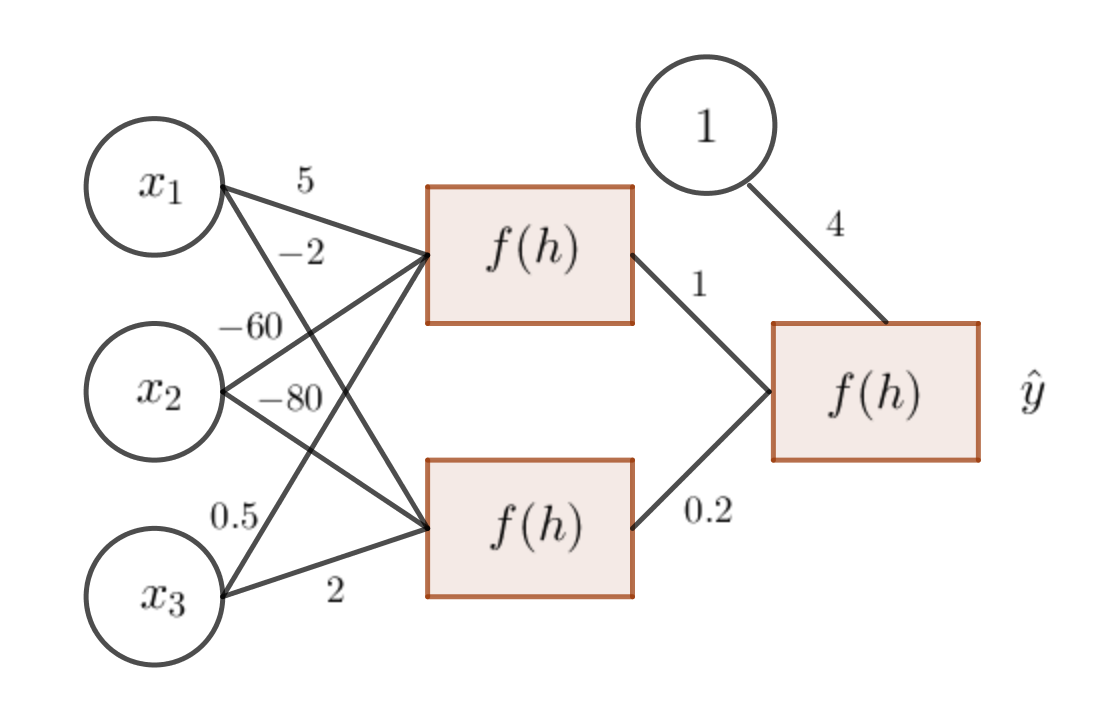
\includegraphics[scale=0.2]{task_1.png}
\end{center}

\begin{enumerate}
\item В эти выходные за барной стойкой стоит Агнесса. Митинга не предвидится, температура будет в районе $20$ градусов. Сколько человек придёт в кофейню к Добродуму? 

\item На самом деле каждая нейросетка --- это просто-напросто какая-то нелинейная сложная функция. Запишите нейросеть Добродума в виде функции.
\end{enumerate}
\end{problem}


\begin{problem}
	Теперь в обратную сторону. Пусть у нас есть вот такая функция. 
	
	\[
	y = \max(0, 4 \cdot \max(0, 3x_1 + 4x_2 + 1) + 2 \cdot \max(0, 3x_1 + 2x_2 + 7) + 6)
	\]
	
	Нарисуйте эту функцию в виде нейросетки. 
\end{problem}


\begin{problem}
	Парни очень любят Свету, а Света любит собирать перцептроны и думать по вечерам об их весах и функциях активации. Сегодня она решила разобрать свои залежи из перцептронов и как следует упорядочить их. 
	
	\begin{itemize}
		
		\item Для перцептрона 
		
		\begin{center}
			\definecolor{cqcqcq}{rgb}{0.7529411764705882,0.7529411764705882,0.7529411764705882}
			\begin{tikzpicture}[line cap=round,line join=round,x=1.0cm,y=1.0cm]
			\clip(-4,1) rectangle (3.306148366367316,4.5);
			\draw [line width=1.pt] (-3.,4.) circle (0.5cm);
			\draw [line width=1.pt] (-3.152000366859971,1.7166134938755313) circle (0.5cm);
			\draw [line width=1.pt] (-1.,3.)-- (-1.,2.);
			\draw [line width=1.pt] (-1.,2.)-- (1.5,2.);
			\draw [line width=1.pt] (1.5,2.)-- (1.5,3.);
			\draw [line width=1.pt] (1.5,3.)-- (-1.,3.);
			\draw [->,line width=1.pt] (-2.5,4.) -- (-1.0315953503775401,2.702352315488771);
			\draw [->,line width=1.pt] (-2.652000366859971,1.7166134938755313) -- (-1.,2.5);
			\draw [->,line width=1.pt] (1.5,2.5) -- (2.5,2.5);
			\draw (-3.4,2) node[anchor=north west] {$x_1$};
			\draw (-0.8,2.8) node[anchor=north west] {$\max(0,t)$};
			\draw (2.6,2.7) node[anchor=north west] {$y$};
			\draw (-1.8,3.9) node[anchor=north west] {$w_1$};
			\draw (-2.5,2.6) node[anchor=north west] {$w_2$};
			\draw (-3.2,4.25) node[anchor=north west] {$1$};
			\end{tikzpicture}
		\end{center}
		
		нужно подобрать веса так, чтобы он превращал $x_1 = 0$ в $y=1$, а $x_1 = 1$ в $y=0$.
		
		\item  Для перцепторона 
		
		\begin{center}
			\begin{tikzpicture}[line cap=round,line join=round,x=1.0cm,y=1.0cm]
			\clip(-4,0.5) rectangle (3.3,4.5);
			\draw [line width=1.pt] (-3.,4.) circle (0.5cm);
			\draw [line width=1.pt] (-3.,2.5) circle (0.5cm);
			\draw [line width=1.pt] (-3.,1.) circle (0.5cm);
			\draw [line width=1.pt] (-1.,3.)-- (-1.,2.);
			\draw [line width=1.pt] (-1.,2.)-- (1.5,2.);
			\draw [line width=1.pt] (1.5,2.)-- (1.5,3.);
			\draw [line width=1.pt] (1.5,3.)-- (-1.,3.);
			\draw [->,line width=1.pt] (-2.5,4.) -- (-1.0315953503775401,2.702352315488771);
			\draw [->,line width=1.pt] (-2.5,2.5) -- (-1.,2.5);
			\draw [->,line width=1.pt] (-2.5,1.) -- (-1.,2.2833448312560893);
			\draw [->,line width=1.pt] (1.5,2.5) -- (2.5,2.5);
			\draw (-3.3,4.25) node[anchor=north west] {$x_1$};
			\draw (-3.3,2.7) node[anchor=north west] {$x_2$};
			\draw (-3.3,1.26) node[anchor=north west] {$x_3$};
			\draw (-0.67, 2.8) node[anchor=north west] {$\max(0,t)$};
			\draw (2.6747622271028213,2.745742538897389) node[anchor=north west] {$y$};
			\draw (-2.1, 4) node[anchor=north west] {$w_1$};
			\draw (-2.25,3) node[anchor=north west] {$w_2$};
			\draw (-2.4,2.1) node[anchor=north west] {$w_3$};
			\end{tikzpicture}
		\end{center}
		
		Света хочет по наблюдениям $x$ подобрать такие веса $w_i$, чтобы на выходе получились $y$. 
		
		\begin{center}
			\begin{tabular}{c|c|c|c}
				$x_1$ & $x_2$ & $x_3$ & $y$ \\
				\hline 
				$1$ & $1$ & $2$ & $0.5$\\
				\hline 
				$1$ & $-1$ & $1$ & $0$ \\
			\end{tabular}
		\end{center}

		
		\item У Светы есть несколько вот таких перцептронов с неизвестной функцией активации (надо самому выбирать):
		
			\begin{center}
			\begin{tikzpicture}[line cap=round,line join=round,x=1.0cm,y=1.0cm]
			\clip(-4,0.5) rectangle (3,4.5);
			\draw [line width=1.pt] (-3.,4.) circle (0.5cm);
			\draw [line width=1.pt] (-3.,2.5) circle (0.5cm);
			\draw [line width=1.pt] (-3.,1.) circle (0.5cm);
			\draw [line width=1.pt] (-1.,3.)-- (-1.,2.);
			\draw [line width=1.pt] (-1.,2.)-- (1.5,2.);
			\draw [line width=1.pt] (1.5,2.)-- (1.5,3.);
			\draw [line width=1.pt] (1.5,3.)-- (-1.,3.);
			\draw [->,line width=1.pt] (-2.5,4.) -- (-1.0315953503775401,2.702352315488771);
			\draw [->,line width=1.pt] (-2.5,2.5) -- (-1.,2.5);
			\draw [->,line width=1.pt] (-2.5,1.) -- (-1.,2.2833448312560893);
			\draw [->,line width=1.pt] (1.5,2.5) -- (2.5,2.5);
			\draw (-3.3,4.25) node[anchor=north west] {$1$};
			\draw (-3.3,2.7) node[anchor=north west] {$x_1$};
			\draw (-3.3,1.26) node[anchor=north west] {$x_2$};
			\draw (-0.2, 2.8) node[anchor=north west] {$f(z)$};
			\draw (2.6747622271028213,2.745742538897389) node[anchor=north west] {$y$};
			\draw (-2.1, 4) node[anchor=north west] {$w_1$};
			\draw (-2.25,3) node[anchor=north west] {$w_2$};
			\draw (-2.4,2.1) node[anchor=north west] {$w_3$};
			\end{tikzpicture}
		\end{center}
	
	На плоскости проведены две прямые $x_1 + x_2 = 1$ и $x_1 - x_2 = 1$. 	
		
		\begin{center}
			\begin{tikzpicture}[line cap=round,line join=round,x=1.0cm,y=1.0cm]
			\clip(-2,-5) rectangle (4,-0.5);
			\draw [line width=2.pt] (-3.,4.) circle (0.5cm);
			\draw [line width=2.pt] (-3.152000366859971,1.7166134938755313) circle (0.5cm);
			\draw [line width=2.pt] (-1.,3.)-- (-1.,2.);
			\draw [line width=2.pt] (-1.,2.)-- (1.5,2.);
			\draw [line width=2.pt] (1.5,2.)-- (1.5,3.);
			\draw [line width=2.pt] (1.5,3.)-- (-1.,3.);
			\draw [->,line width=2.pt] (-2.5,4.) -- (-1.0315953503775401,2.702352315488771);
			\draw [->,line width=2.pt] (-2.652000366859971,1.7166134938755313) -- (-1.,2.5);
			\draw [->,line width=2.pt] (1.5,2.5) -- (2.5,2.5);
			\draw (-3.270567410142784,1.9563548477920916) node[anchor=north west] {$x_1$};
			\draw (-0.17178835933248715,2.8036772444980356) node[anchor=north west] {$\max(0,t)$};
			\draw (2.6727939724660277,2.7552588218291243) node[anchor=north west] {$y$};
			\draw (-1.7695963074065464,3.8809871488813075) node[anchor=north west] {$w_1$};
			\draw (-2.217466717093972,2.6342127651568465) node[anchor=north west] {$w_2$};
			\draw (-3.088998325134368,4.2562299245653685) node[anchor=north west] {$1$};
			\draw [->,line width=2.pt] (1.,-5.) -- (1.,-1.);
			\draw [->,line width=2.pt] (-2.,-3.) -- (4.,-3.);
			\draw (2.0191452664357303,-1.251365654023268) node[anchor=north west] {$1$};
			\draw (-0.3170436273392198,-2.4134077980771345) node[anchor=north west] {$0$};
			\draw [line width=2.pt,dash pattern=on 3pt off 3pt] (0.,-5.)-- (4.,-1.);
			\draw [line width=2.pt,dash pattern=on 3pt off 3pt] (0.,-1.)-- (4.,-5.);
			\draw (1.910203815430681,-4.0112157461512) node[anchor=north west] {$0$};
			\draw (3.2417104388257303,-2.4013031924099066) node[anchor=north west] {$0$};
			\end{tikzpicture}
		\end{center}
	
	Свете нужно собрать нейросетку, которая будет классифицировать объекты с плоскости так, как показано на картинке.
	\end{itemize}
\end{problem}



\begin{problem}

Есть теорема, которая говорит о том, что с помощью нейросетки можно аппроксимировать почти любую функцию. Попробуйте с помощью нейросеток с минимально возможным числом нейронов описать логический функции, заданные следующими таблицами истинности: 

\begin{center}
\begin{minipage}{0.3\linewidth} 
	\begin{tabular}{c|c|c}
	$x_1$ & $x_2$ & $x_1 \cap x_2$ \\
	\hline 
	$1$ & $1$ & $1$ \\
	\hline 
	$1$ & $0$ & $0$ \\
	\hline 
	$0$ & $1$ & $0$ \\
	\hline 
	$0$ & $0$ & $0$ \\
\end{tabular}
\end{minipage}
\hfill
\begin{minipage}{0.3\linewidth}
		\begin{tabular}{c|c|c}
		$x_1$ & $x_2$ & $x_1 \cup x_2$ \\
		\hline 
		$1$ & $1$ & $1$ \\
		\hline 
		$1$ & $0$ & $1$ \\
		\hline 
		$0$ & $1$ & $1$ \\
		\hline 
		$0$ & $0$ & $0$ \\
	\end{tabular}
\end{minipage}
\hfill
\begin{minipage}{0.3\linewidth}
		\begin{tabular}{c|c|c}
		$x_1$ & $x_2$ & $x_1 \mbox{ } XoR \mbox{ } x_2$ \\
		\hline 
		$1$ & $1$ & $0$ \\
		\hline 
		$1$ & $0$ & $1$ \\
		\hline 
		$0$ & $1$ & $1$ \\
		\hline 
		$0$ & $0$ & $0$ \\
	\end{tabular}
\end{minipage}
\end{center}

Первые два столбика идут на вход, третий получается на выходе.  Операция из третьей таблицы называется исключающим или.  
\end{problem}


\begin{problem}

Сколько минимально нейронов необходимо для решения следующих двух задач классификации?  Сколько слоёв минимально должно быть в нейросетке?  Почему?  

\begin{center}
	\definecolor{qqqqff}{rgb}{0.,0.,1.}
	\definecolor{qqwuqq}{rgb}{0.,0.39215686274509803,0.}
	\begin{tikzpicture}[scale = 0.7, line cap=round,line join=round,x=1.0cm,y=1.0cm]
	\clip(-5.5,1) rectangle (9,7);
	\draw [line width=2.pt] (1.,7.)-- (1.02,1.8);
	\begin{scriptsize}
	\draw [fill=qqwuqq] (-2.6,4.9) circle (2.5pt);
	\draw [fill=qqwuqq] (-2.,4.) circle (2.5pt);
	\draw [fill=qqwuqq] (-1.42,4.9) circle (2.5pt);
	\draw [fill=qqqqff] (-0.44,5.84) circle (2.5pt);
	\draw [fill=qqqqff] (-1.52,5.9) circle (2.5pt);
	\draw [fill=qqqqff] (-3.,6.) circle (2.5pt);
	\draw [fill=qqqqff] (-4.02,5.7) circle (2.5pt);
	\draw [fill=qqqqff] (-3.36,4.28) circle (2.5pt);
	\draw [fill=qqqqff] (-2.4,2.92) circle (2.5pt);
	\draw [fill=qqqqff] (-1.18,3.38) circle (2.5pt);
	\draw [fill=qqqqff] (-0.56,4.16) circle (2.5pt);
	\draw [fill=qqqqff] (0.,5.) circle (2.5pt);
	\draw [fill=qqqqff] (-3.52,3.32) circle (2.5pt);
	\draw [fill=qqqqff] (-0.44,2.5) circle (2.5pt);
	\draw [fill=qqqqff] (-1.44,2.78) circle (2.5pt);
	\draw [fill=qqqqff] (0.06,6.38) circle (2.5pt);
	\draw [fill=qqqqff] (-2.96,6.78) circle (2.5pt);
	\draw [fill=qqqqff] (-4.02,4.56) circle (2.5pt);
	\draw [fill=qqwuqq] (-2.06,4.62) circle (2.5pt);
	\draw [fill=qqwuqq] (-2.,5.) circle (2.5pt);
	\draw [fill=qqwuqq] (-1.72,4.4) circle (2.5pt);
	\draw [fill=qqwuqq] (-2.46,4.42) circle (2.5pt);
	\draw [fill=qqqqff] (-2.22,6.26) circle (2.5pt);
	\draw [fill=qqqqff] (1.84,5.84) circle (2.5pt);
	\draw [fill=qqqqff] (1.84,4.86) circle (2.5pt);
	\draw [fill=qqqqff] (1.84,3.62) circle (2.5pt);
	\draw [fill=qqqqff] (1.84,2.62) circle (2.5pt);
	\draw [fill=qqqqff] (2.68,2.56) circle (2.5pt);
	\draw [fill=qqqqff] (2.68,3.38) circle (2.5pt);
	\draw [fill=qqqqff] (2.54,4.5) circle (2.5pt);
	\draw [fill=qqqqff] (2.64,5.72) circle (2.5pt);
	\draw [fill=qqqqff] (5.04,5.6) circle (2.5pt);
	\draw [fill=qqqqff] (5.,4.56) circle (2.5pt);
	\draw [fill=qqqqff] (4.92,3.36) circle (2.5pt);
	\draw [fill=qqqqff] (4.92,2.48) circle (2.5pt);
	\draw [fill=qqqqff] (5.98,2.32) circle (2.5pt);
	\draw [fill=qqqqff] (5.98,3.16) circle (2.5pt);
	\draw [fill=qqqqff] (6.,4.) circle (2.5pt);
	\draw [fill=qqqqff] (5.94,4.76) circle (2.5pt);
	\draw [fill=qqqqff] (5.92,5.34) circle (2.5pt);
	\draw [fill=qqwuqq] (3.42,5.12) circle (2.5pt);
	\draw [fill=qqwuqq] (3.44,5.94) circle (2.5pt);
	\draw [fill=qqwuqq] (4.28,5.8) circle (2.5pt);
	\draw [fill=qqwuqq] (4.28,5.3) circle (2.5pt);
	\draw [fill=qqwuqq] (3.54,3.98) circle (2.5pt);
	\draw [fill=qqwuqq] (4.,4.) circle (2.5pt);
	\draw [fill=qqwuqq] (3.5,2.98) circle (2.5pt);
	\draw [fill=qqwuqq] (4.18,2.94) circle (2.5pt);
	\draw [fill=qqwuqq] (3.4,2.32) circle (2.5pt);
	\draw [fill=qqwuqq] (4.18,2.36) circle (2.5pt);
	\draw [fill=qqwuqq] (3.98,4.56) circle (2.5pt);
	\end{scriptsize}
	\end{tikzpicture}
\end{center}
\end{problem}

\newpage

\begin{problem}
Доказать, что с помощью однослойной нейронной сетки можно приблизить любую непрерывную функцию от одного аргумента $f(x)$ со сколь угодно большой точностью\footnote{\url{http://neuralnetworksanddeeplearning.com/chap4.html}}.  

\textbf{Hint:}  Вспомните, что любую непрерывную функцию можно приблизить с помощью кусочно-линейной функции (ступеньки). Осознайте как с помощью пары нейронов можно описать такую ступеньку. Соедините все ступеньки в сумму с помощью выходного нейрона. 
\end{problem}


\begin{problem}
	Маша услышала про машин лёрнинг и решила, что они и есть та самая Маша, которой этот лёрнинг принадлежит. Теперь она собирается обучить нейронную сеть для решения задачи регрессии, На вход в неё идёт $12$ переменных, в сетке есть $3$ скрытых слоя. В пером слое $300$ нейронов, во втором $200$, в третьем $100$. 
	
	\begin{itemize}
		\item[a)] Сколько параметров предстоит оценить Маше?  Сколько наблюдений вы бы на её месте использовали? 
		\item[b)] Пусть в каждом слое была отключена половина нейронов. Сколько коэффициентов необходимо оценить?
		\item[c)] Предположим, что Маша решила после первого слоя добавить в свою сетку Dropout c вероятностью $p$.  Какова вероятность того, что отключится весь слой? 
		\item[d)] Маша добавила Dropout c вероятностью $p$. после каждого слоя. Какова вероятность того, что один из слоёв отключится и сетка не сможет учиться? 
		\item[e)] Пусть случайная величина $N$ --- это число включённых нейронов. Найдите её математическое ожидание и дисперсию. Если Маша хочет проредить сетку на четверть, какое значение $p$ она должна поставить? 
		\item[f)] Пусть случайная величина $P$ --- это число параметров в нейросети, которое необходимо оценить. Найдите её математическое ожидание и дисперсию. Почему найденное вами математическое ожидание выглядит очень логично? Что оно вам напоминает? Обратите внимание на то, что смерть одного из параметров легко может привести к смерти другого.
	\end{itemize}
\end{problem}


\begin{problem}
	Та, в чьих руках находится лёрнинг (это Маша), решила немного поэкспериментировать с выходами из своей сетки. 
	\begin{itemize}
		\item[a)]  Для начала Маша решила, что хочет решать задачу классификации на два класса и получать на выходе вероятность принадлежности к первому. Что ей надо сделать с последним слоем сетки? 
		\item[b)]  Теперь Маша хочет решать задачу классификации на $K$ классов. Что ей делать с последним слоем? 
		\item[c)]  Новые вводные! Маша хочет спрогнозировать рейтинг фильма на "Кинопоиске". Он измеряется по шкале от $0$ до $10$ и принимает любое непрерывное значение. Как Маша может приспособить для этого свою нейронку? 
		\item[d)]  У Маши есть куча новостей. Каждая новость может быть спортивной, политической или экономической. Иногда новость может относится сразу к нескольким категориям. Как Маше собрать нейросетку для решения этой задачи?  Как будет выглядеть при этом функция ошибки? 
		\item[e)]  Маша пошла в кафе. А там куча народу. Сейчас она сидит за столиком, попивает ванильный топлёный кортадо и думает о нём, о лёрнинге.  Сейчас мысль такая: как можно спрогнозировать число людей в кафе так, чтобы на выходе сетка всегда прогнозировала целое число. Надо ли как-то при этом менять функцию потерь? 
		% \item[f)] Пункт с регрессией и весами из денег 
	\end{itemize}
\end{problem}


%\begin{problem}
%  Сделать задачу по связи ранней остановки и регуляризатора 
%\end{problem}

\section*{Ещё задача}

Если вы никогда не решали эту задачку, рекомендую сделать это. Она довольно неплохо открывает чакру на работу с регуляризаторами, и показывает как именно они стягивают к нулю коэффициенты, не давая модели переобучаться. В рамках нейросеток механизм точно такой же. 

\begin{problem}
	Вася измерил вес трёх покемонов,  $y_1=6$, $y_2=6$, $y_3=10$.  Вася хочет спрогнозировать вес следующего покемона. Модель для веса покемонов у Васи очень простая, $y_i = \beta + \varepsilon_i$, поэтому прогнозирует Вася по формуле $\hat y_i = \hat \beta$.
	
	Для оценки параметра $\beta$ Вася использует следующую целевую функцию:
	
	\[
	\sum (y_i - \hat \beta)^2 + \lambda \cdot \hat \beta^2
	\]
	
	\begin{enumerate}
		\item[a)] Найдите оптимальное $\hat \beta$ при $\lambda =0$.
		\item[б)] Найдите оптимальное $\hat \beta$ при произвольном $\lambda$. Правда ли, что чем больше $\lambda$, тем меньше $\beta$? 
		\item[в)] Подберите оптимальное $\lambda$ с помощью кросс-валидации leave one out («выкинь одного»). При такой валидации на первом шаге мы оцениваем модель на всей выборке без первого наблюдения, а на первом тестируем её. На втором шаге мы оцениваем модель на всей выборке без второго наблюдения, а на втором тестируем её. И так далее $n$ раз. Каждое наблюдение является отдельным фолдом.
		\item[г)] Найдите оптимальное $\hat \beta$ при $\lambda_{CV}$.
	\end{enumerate}
\end{problem}




\end{document}